\documentclass[	11pt, ]{fphw}

\usepackage[utf8]{inputenc} 
\usepackage[T1]{fontenc}
\usepackage{mathpazo}\usepackage{graphicx} 
\usepackage{booktabs} 
\usepackage{listings} 
\usepackage{amsmath}
\usepackage{eso-pic}
\usepackage{array}
\usepackage{float}
\usepackage{graphicx}
\usepackage{bbm}
\usepackage{transparent}
\usepackage{indentfirst}
\usepackage{amsthm}
\usepackage{amsmath,amssymb}
\usepackage{subfigure}
\usepackage{tabu}
\usepackage{enumitem}
\usepackage{caption,tabularx,booktabs}
\usepackage{enumerate} 
\usepackage[english]{varioref}

\renewcommand{\thesection}{\Roman{section}}
\usepackage{titlesec}
\titleformat{\section}
{\normalfont\Large\bfseries}{Exercise~\thesection}{1em}{}
\makeatletter
\renewcommand{\@seccntformat}[1]{%
  \csname the#1\endcsname
  \csname suffix@#1\endcsname % this does nothing unless \suffix@... is defined
  \quad
}
% the subsection number is just a letter
\renewcommand{\thesubsection}{\alph{subsection}}
% but references will also have “section.subsection.” in front of the letter
\renewcommand{\p@subsection}{\thesubsection.}
% define \suffix@subsection
\newcommand{\suffix@subsection}{)}
\makeatother

\title{Assignment \#4} %
\author{Anita Mezzetti} 
\institute{École polytechnique fédérale de Lausanne} 
\class{Global Business Environment} 
\professor{Luisa Lambertini} 

%--------------------------------------------------------------------
\begin{document}
\maketitle 
\section{}
False. \\
"The Federal Reserve System is the Central Bank of the United States. It performs five general functions to promote the effective operation of the U.S. economy and, more generally, the public interest. The Federal Reserve conducts the nation’s monetary policy to promote maximum employment, stable prices, and moderate long-term interest rates in the U.S. economy. It promotes the stability of the financial system and seeks to minimize and contain systemic risks through active monitoring and engagement in the U.S. and abroad. The Federal Reserve promotes the safety and soundness of individual financial institutions and monitors their impact on the financial system as a whole. It fosters payment and settlement system safety and efficiency through services to the Banking industry and the U.S. government that facilitate U.S.-dollar transactions and payments. Finally it promotes consumer protection and community development through consumer-focused supervision and examination, research and analysis of emerging consumer issues and trends, community economic development activities, and the administration of consumer laws and regulations.". \cite{res}
\par 
The Fed's objective is to have the inflation of 2$\%$, so currently it is “running below” the target. The fact that inflation is above or below target influences interest rates.
Moreover, we should consider that exogenous factors can influence the decision of the Fed. Between them we can mention the tensions with China and the Brexit. It is a fact that data increasingly suggest that a slowdown is materializing. So Fed officials have reasons to keep their options open. For example, Fed can consider the potential for a coming cut of interest rates given risks to the U.S. economic outlook; always remembering that the goal is to to sustain a low unemployment rate, solid growth and stable inflation. 
\newpage
\section{}
\subsection{}
We have a temporary decrease in aggregate real money abroad. Then we know that the foreign Central Bank accommodates the reduction in money demand and that the foreign interest rate is unchanged. A reduction in money demand corresponds to a reduction in money supply. So,we do not have any impact on the exchange rate and there are not short run domestic effects. See Figure \vref{11}.

\begin{figure}[h] 
\centering 
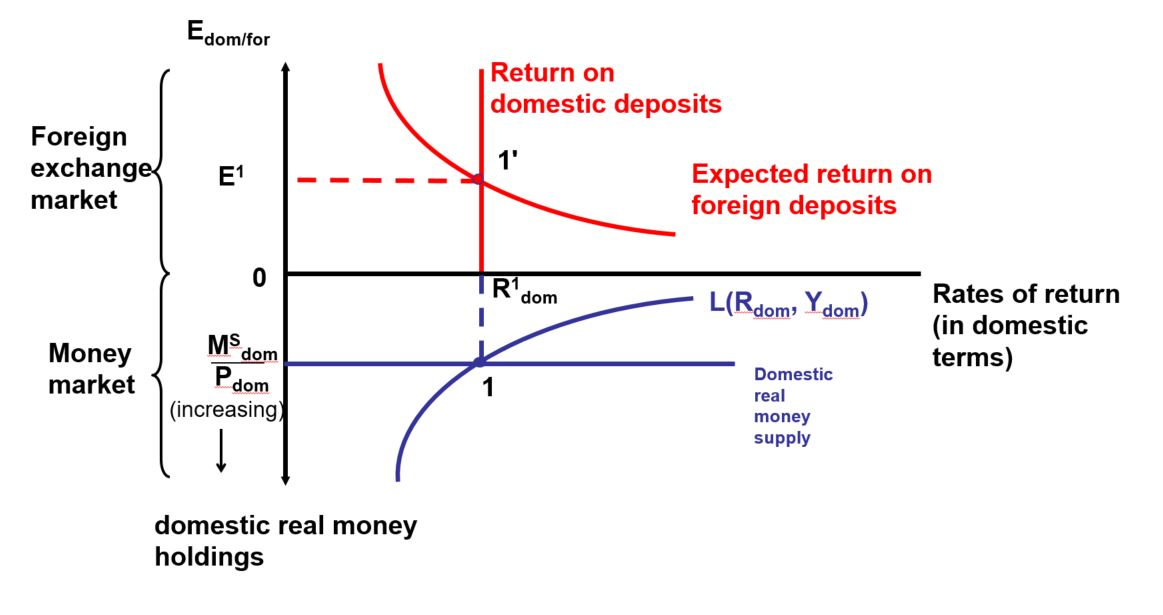
\includegraphics[scale=0.75]{11.JPG} 
\caption{(Question 2.a) Short run effect of the reduction in money demand and foreign interest rate unchanged.} 
\label{11}
\end{figure}

\subsection{}
We have a temporary decrease in aggregate real money abroad. Then we know that the foreign Central Bank leaves foreign money supply unchanged. That means that we have a situation where the foreign equilibrium interest rate has to decrease, to compensate the decrease in aggregate real money abroad. See figure \vref{21}. A decrease of R$_{for}$ leads to a decrease in E$_{dom/for}$. In fact we have
\[ R_{dom}= R_{for} + \frac{E_{dom/for}^{e}}{E_{dom/for}} -1. \]
The Figure \vref{22} explains the domestic economy, which is affected by the fall of E$_{dom/for}$ (appreciation of the domestic currency). The equilibrium point moves from point 1 to point 2. 


\begin{figure}[h!] 
\centering 
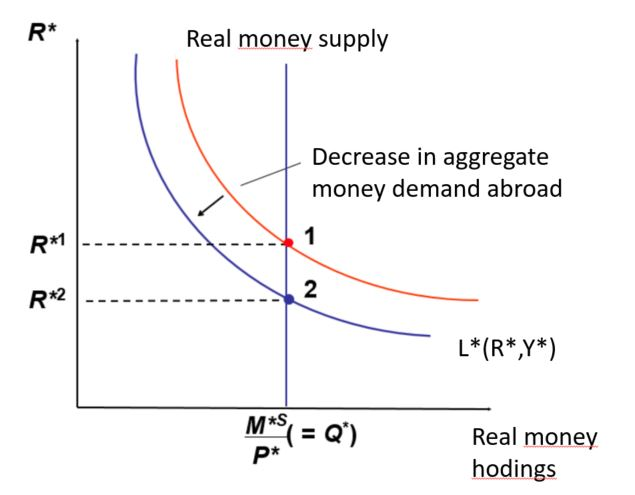
\includegraphics[scale=0.7]{21.JPG} 
\caption{(Question 2.b) Effects on the foreign interest rate when there is a temporary decrease in aggregate real money abroad. } 
\label{21}
\end{figure}


\begin{figure}[h] 
\centering 
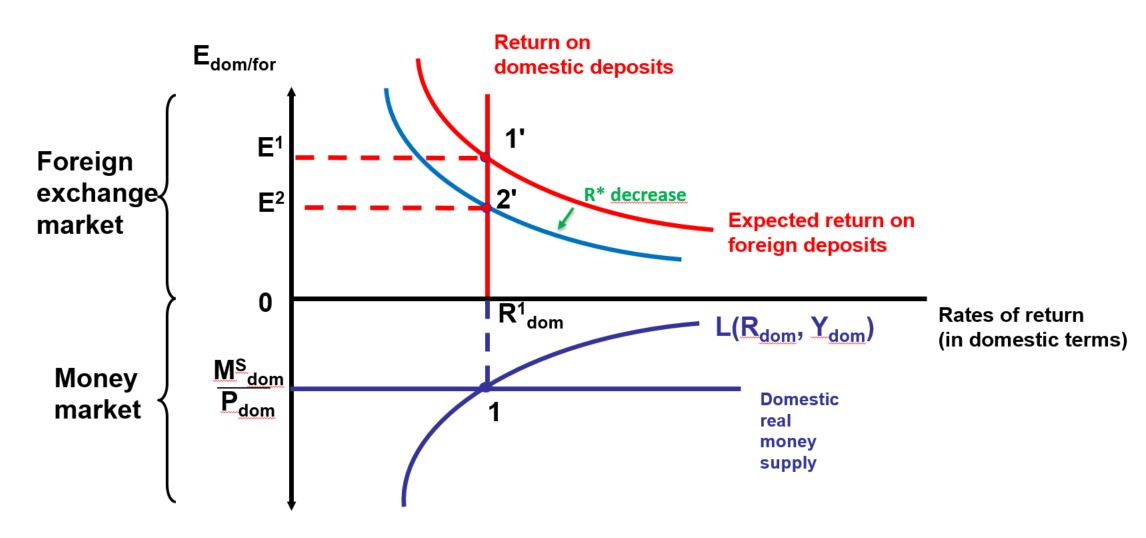
\includegraphics[scale=0.75]{22.JPG} 
\caption{(Question 2.b) Short run effect of the reduction in money demand and foreign money supply rate unchanged.} 
\label{22}
\end{figure}

\section{}
\subsection{}
If we have equilibrium, the money demand is equal to the money supply. 
\begin{align}
    M_{CHF}^{s}/P_{CHF} = & L ( R_{CHF}, Y_{CHF} ) \\
    400/1 =& 300+1,02 x Y_{CHF}- 100 x R_{CHF} \\
    400/1 =& 300+1,02 x 100 - 100x R_{CHF} \\
    R_{CHF} =&  0.02
\end{align}

\subsection{}
\[ R_{CHF}= R_{EUR} + \frac{E_{CHF/EUR}^{e}}{E_{CHF/EUR}} -1. \]
So,
\[ E_{CHF/EUR} = \frac{E_{CHF/EUR}^{e}}{1+R_{CHF}-R_{EUR}}= \frac{1,21}{1+0,02-0,05}=1,247 \]



\subsection{}
Central Bank can decide not to accommodate the change in domestic money demand and it compensates through a decrease of the R$_{CHF}$. In this way there is a new R$^{2}_{CHF}$, which represents the point of equilibrium. In this way also the E$_{CHF/EUR}$ would change: it would increase (depreciation of domestic currency). This case is explained in Figure \vref{32}.

\begin{figure}[h] 
\centering 
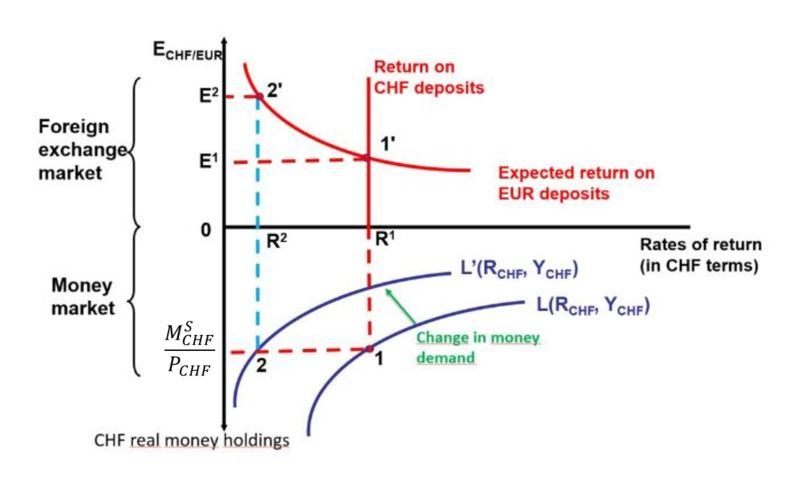
\includegraphics[scale=0.85]{32.JPG} 
\caption{(Question 3.c) Short-run equilibrium if money demand temporarily changes and the domestic Central Bank does not accommodate the change in domestic money demand. } 
\label{32}
\end{figure}

\subsection{}
We suppose that the domestic interest rate changes, while the money supply remains the same: 
\begin{align}
    M_{CHF}^{s}/P_{CHF} = & L ( R_{CHF}, Y_{CHF} ) \\
400/1= & 300 + 1 x  Y_{CHF} - 100 x R_{CHF} \\
R_{CHF} =0.
\end{align}
R$_{CHF}$ is the new equilibrium interest rate. In this case also the rate of return change: 
\begin{align}
 R_{CHF}= & R_{EUR} + \frac{E_{CHF/EUR}^{e}}{E_{CHF/EUR}} -1 \\
0   = & 0,05+ \frac{1,21}{E_{CHF/EUR}} -1 \\
E_{CHF/EUR}= & \frac{1,21}{1-0,05} \\
E_{CHF/EUR}= & 1,2737
\end{align}

\newpage 

\subsection{}
If the Central Bank decides to accommodate the change in in domestic money demand, it has to change the money supply. The Central Bank leaves the equilibrium R$_{CHF}$ unchanged.
In this case, as it is explained in Figure \vref{31}, there is a decrease in money supply.
The money supply decreases to restore the equilibrium. The R$_{CHF}$ remain unchanged, so there is not a short run effect on exchange rate.

\begin{figure}[h] 
\centering 
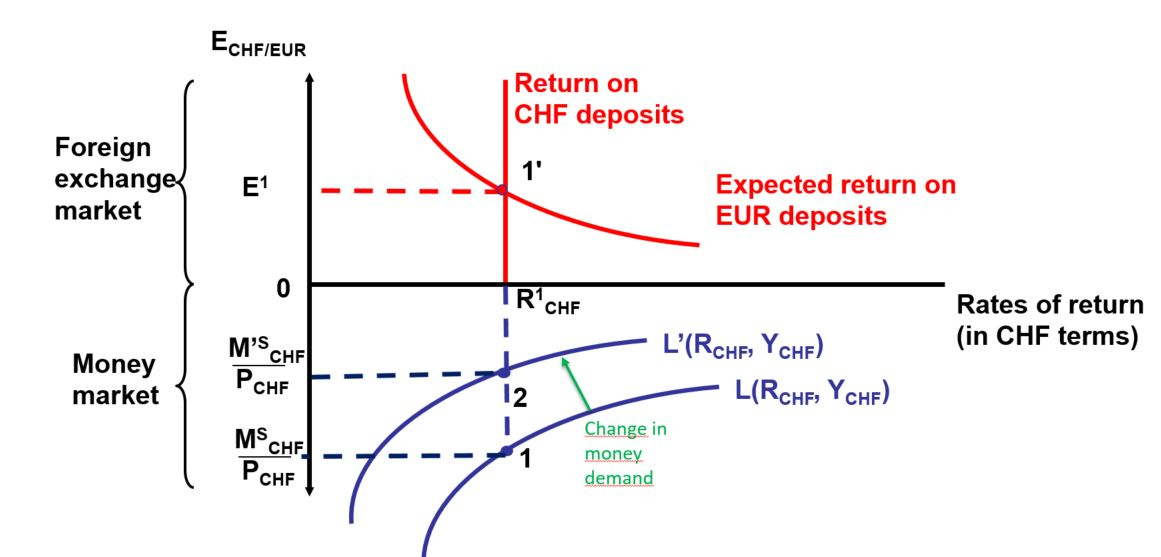
\includegraphics[scale=0.75]{31.JPG} 
\caption{(Question 3.e) Short-run equilibrium if money demand temporarily changes and the domestic Central Bank accommodates the change in domestic money demand.} 
\label{31}
\end{figure}

\subsection{}
\[ M_{CHF}^{2s}/P_{CHF} = L' ( R_{CHF}, Y_{CHF} ) \]
\[  M_{CHF}^{2s}=P_{CHF}x( L' ( R_{CHF}, Y_{CHF} ))= 300+1x100-100x0.02=398. \]
The R$_{CHF}$ remains unchanged, so there is not a short run effect on exchange rate.
\\
\begin{thebibliography}{99}
\bibitem{res} Overview of the Federal Reserve System;
\end{thebibliography}























\end{document}